\section{Auswertung}
\label{sec:Auswertung}

% Messwerte: Alle gemessenen physikalischen Größen sind übersichtlich darzustellen.

% Auswertung:
% Berechnung der geforderten Endergebnisse
% mit allen Zwischenrechnungen und Fehlerformeln, sodass die Rechnung nachvollziehbar ist.
% Eine kurze Erläuterung der Rechnungen (z.B. verwendete Programme)
% Graphische Darstellung der Ergebnisse

\subsection{Bestimmung der Zeitkonstante}
\label{sec:Auswertung_Zeitkonstante}

Im ersten Teil des Versuchs wie in \autoref{sec:Durchführung_1} konnte nur ein Foto der Entladekurve als Messergebnis dienen, dieses ist in \autoref{fig:foto_entladekurve} dargestellt:

\begin{figure}
    \centering
    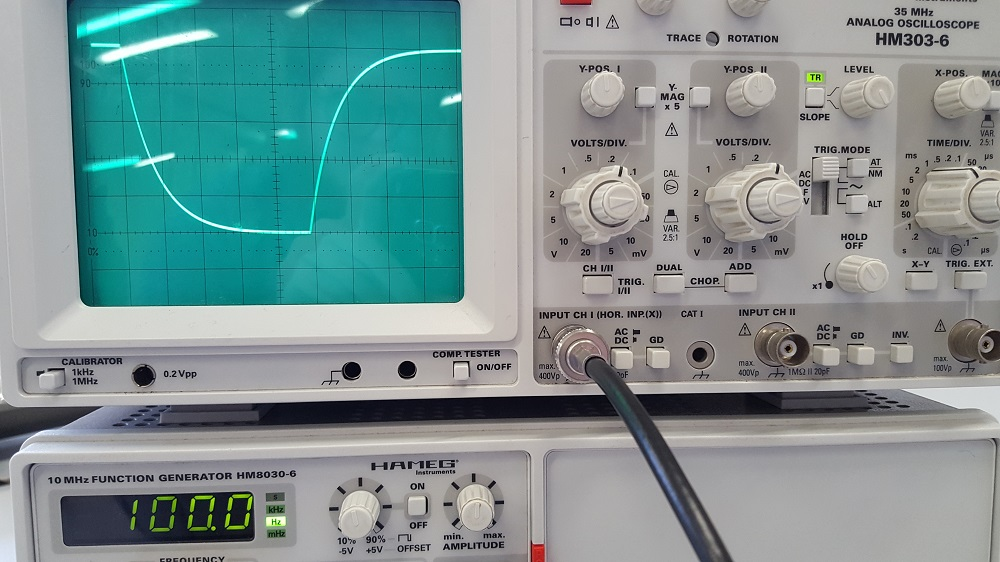
\includegraphics[width=\textwidth]{images/foto_01.jpg}
    \caption{Foto der Entladekurve des RC Glieds bei angeschlossener Rechteckspannung mit $\SI{100}{\hertz}$}
    \label{fig:foto_entladekurve}
\end{figure}

\subsection{Untersuchung bei einer angelegten Sinusspannung}
\label{sec:Auswertung_Sinusspannung}

Die Ergebnisse der im \autoref{sec:Durchführung_2} beschriebenen Durchführung sind in \autoref{tab:gemessen} dargestellt. Hierbei ist zu beachten, dass die Werte $a$ bei einer invertierten Generatorspannung abgelesen wurden. Also entspricht der zeitliche Abstand $a$ der Zeit zwischen steigendem Nulldurchgang der Kondensatorspannung und abfallendem Nulldurchgang der Generatorspannung.

\begin{table}
    \centering
    \caption{Messergebnisse zu \autoref{sec:Durchführung_2} mit Generatorfrequenz $f$, Kondensatorspannung $U_C$, zeitlicher Abstand $a$ (siehe Beschreibung)}
    \label{tab:gemessen}
    \begin{tabular}{c c c}
        \toprule
        $f \:/\: \si{\hertz}$ & $U_C \:/\: \si{\volt}$ & $a \:/\: \si{\milli\second}$ \\
        \midrule
        20 & 1.000 & 25.000 \\
        50 & 0.960 & 9.200 \\
        100 & 0.900 & 4.200 \\
        200 & 0.700 & 1.850 \\
        300 & 0.550 & 1.150 \\
        400 & 0.450 & 0.800 \\
        500 & 0.360 & 0.620 \\
        600 & 0.300 & 0.500 \\
        800 & 0.240 & 0.360 \\
        1000 & 0.200 & 0.280 \\
        2000 & 0.100 & 0.130 \\
        3000 & 0.067 & 0.085 \\
        4500 & 0.044 & 0.056 \\
        6000 & 0.034 & 0.042 \\
        10000 & 0.020 & 0.025 \\
        \bottomrule
    \end{tabular}
\end{table}

\subsection{Betrachtung des RC-Glieds als Integrator}
\label{sec:Auswertung_Integrator}

Im letzten Teil des Versuchs wie in \autoref{sec:Durchführung_3} beschrieben sind die Ergebnisse nur in Form von Fotos darzustellen. Diese sind in \autoref{fig:fotos_integrator} zu sehen. Hierbei wurde jeweils die Generatorfrequenz von $\SI{5}{\kilo\hertz}$ gewählt.

\begin{figure}
    \centering
    \begin{subfigure}{0.3\textwidth}
        \centering
        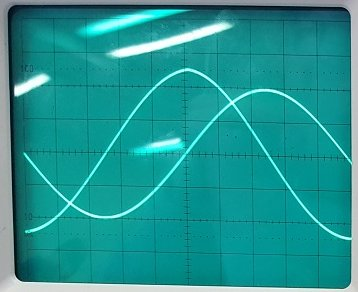
\includegraphics[height=3.3cm]{images/foto_03_ausschnitt.jpg}
        \caption{Sinusspannung}
        \label{fig:foto_sin_integrator}
    \end{subfigure}
    \begin{subfigure}{0.3\textwidth}
        \centering
        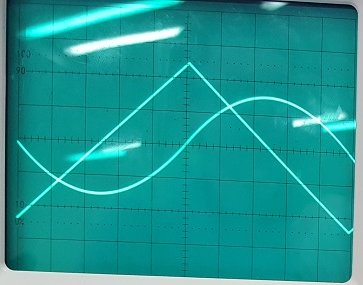
\includegraphics[height=3.3cm]{images/foto_04_ausschnitt.jpg}
        \caption{Sägezahnspannung}
        \label{fig:foto_saege_integrator}
    \end{subfigure}
    \begin{subfigure}{0.3\textwidth}
        \centering
        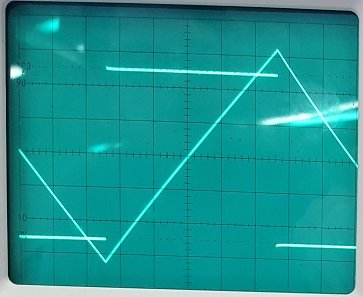
\includegraphics[height=3.3cm]{images/foto_05_ausschnitt.jpg}
        \caption{Rechteckspannung}
        \label{fig:foto_rechteck_integrator}
    \end{subfigure}
    \caption{Fotos der Integratorschaltung für eine Generatorfrequenz von $\SI{5}{\kilo\hertz}$ und verschiedene Generatorspannungstypen}
    \label{fig:fotos_integrator}
\end{figure}